\usetikzlibrary{matrix}
\begin{frame}{autoconfiguration}
    \begin{itemize}
    \item how do hosts get address + default routing table?
    \item one answer: set manually
    \end{itemize}
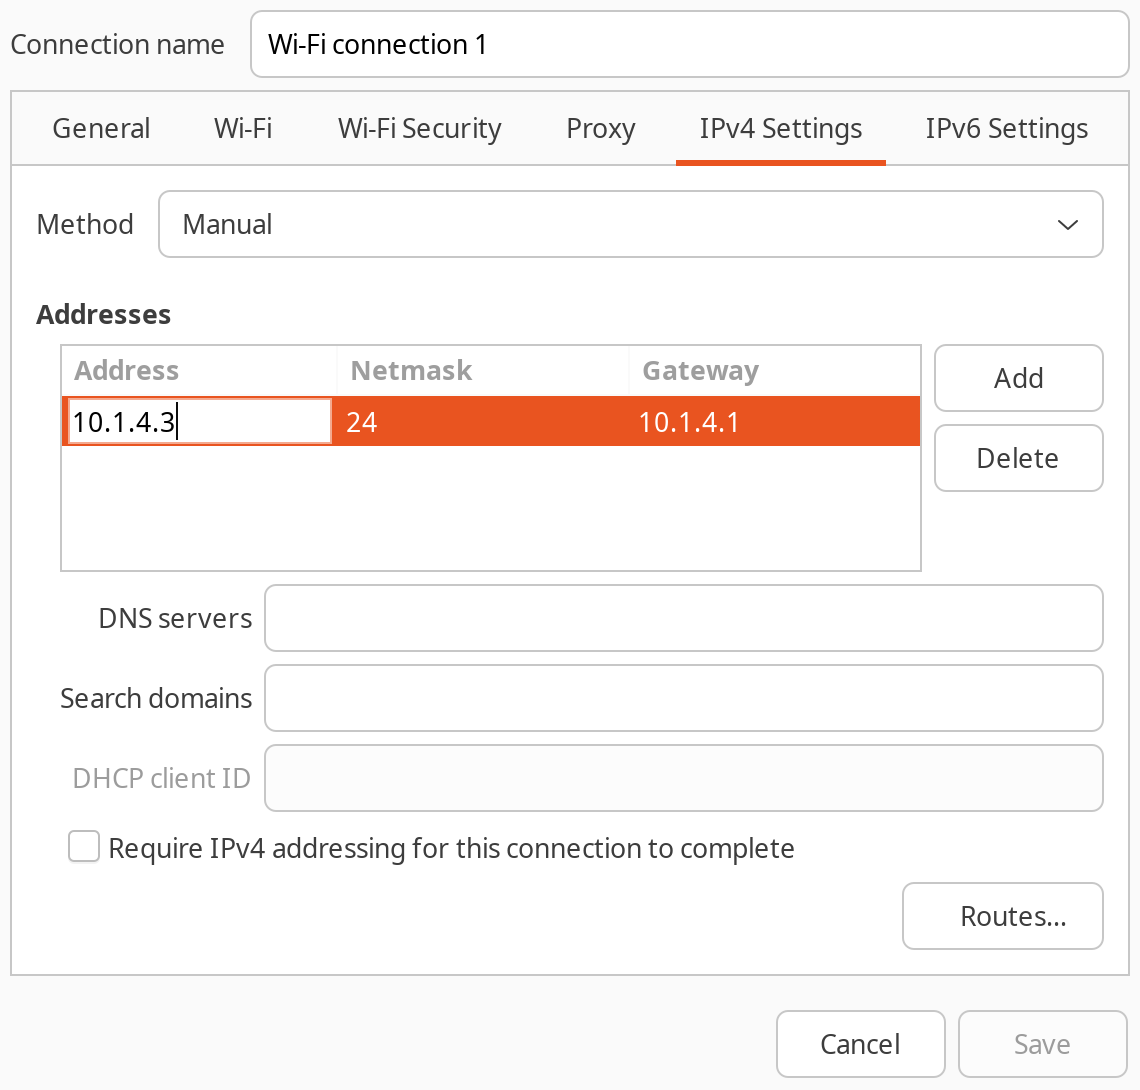
\includegraphics[width=0.5\textwidth]{../arp/ip-config-dialog}
\end{frame}

\begin{frame}{simple network config}
\begin{itemize}
    \item IP address: 10.0.2.45
    \item (sub)net mask: /25 (aka 255.255.255.128)
        \begin{itemize}
        \item varies which format is input
        \end{itemize}
    \item (default) gateway: 10.0.2.102
\end{itemize}
\begin{visibleenv}<2->
\begin{tikzpicture}
\matrix[tight matrix,
    nodes={minimum height=0.4cm},
    column 1/.style={nodes={text width=4cm}},
    column 2/.style={nodes={text width=3cm}},
    column 3/.style={nodes={text width=2cm}},
] {
addresses \& next hop \& device \\
10.2.0.0/25 \& (direct) \& out \\
default \& 10.2.0.102 \& out \\
};
\end{tikzpicture}
\end{visibleenv}
\end{frame}

\begin{frame}{DHCP messages (1)}
    \begin{itemize}
    \item protocol looks weird in packet traces because of history
    \item built on top of UDP + IP
    \item built as extension to older BOOTP (bootstrap protocol)
    \vspace{.5cm}
    \item common message format for different ``operations''
    \end{itemize}
\end{frame}

\begin{frame}{DHCP messages (2)}
    \begin{itemize}
    \item from client (looking to configure itself):
        \begin{itemize}
        \item DISCOVER (look for configuration server)
        \item REQUEST (get configuration from server)
        \end{itemize}
    \item from server (offering configurations):
        \begin{itemize}
        \item OFFER (`I am a configuration server')
        \item ACK (here's a configuration)
        \end{itemize}
    \end{itemize}
\end{frame}

\begin{frame}[fragile]{DHCP request example}
\begin{tikzpicture}
\tikzset{
    explain box/.style={draw=red,ultra thick,fill=white,align=left},
    hi box/.style={draw=red,line width=1mm},
}
\node[inner sep=0mm,anchor=north west] at (0, 0) {%
    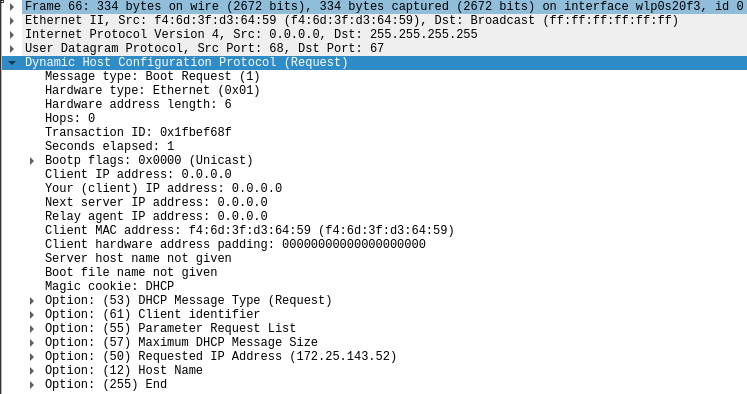
\includegraphics[width=\textwidth]{../arp/dhcp-request-wireshark.png}%
};
%\path[overlay,draw,help lines] (0, 0) grid (15, -8);
\begin{visibleenv}<2>
    \path[hi box] (0.4, -0.2) rectangle (13.2, -1.25);
    \node[anchor=north,explain box] at (7, -1.5) {
        built on IP+UDP rather than special protocol like ARP \\
        ~ \\
        sending to broadcast ethernet/IP address (all 1 bits)\\
        placeholder source IP of 0.0.0.0
    };
\end{visibleenv}
\begin{visibleenv}<3>
    \path[hi box] (0.5, -1.3) rectangle (5.2, -1.7);
    \node[anchor=north,explain box] at (8, -1.8) {
       `boot' probably because derived \\ from bootstrap protocol (BOOTP)
    };
\end{visibleenv}
\begin{visibleenv}<4>
    \path[hi box] (0.5, -3.2) rectangle (8.8, -4.6);
    \node[anchor=north,explain box] at (7, -5) {
        message format same in both directions, so \\
        fields here intended for use in response
    };
\end{visibleenv}
\end{tikzpicture}
\end{frame}

\begin{frame}{DHCP ACK example}
\begin{tikzpicture}
\tikzset{
    explain box/.style={draw=red,ultra thick,fill=white,align=left},
    hi box/.style={draw=red,line width=1mm},
}
\node[anchor=north west,inner sep=0mm] at (0, 0) {%
    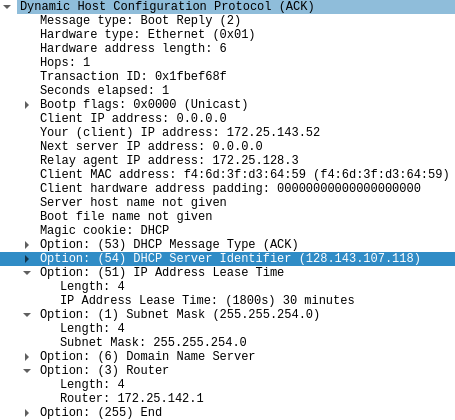
\includegraphics[width=0.55\textwidth]{../arp/dhcp-response3-wireshark.png}
};
%\path[overlay,draw,help lines] (0, 0) grid (15, -8);
\begin{visibleenv}<2>
    \draw[hi box] (0.6, -2.1) rectangle (5.7, -2.45);
    \draw[hi box] (0.6, -2.6) rectangle (5.5, -3.0);
    \draw[hi box] (0.4, -4.1) rectangle (7.5, -7.5);
    \node[explain box,anchor=north east] at (15, -2) {
        response (ACK) has address fields filled in
    };
\end{visibleenv}
\begin{visibleenv}<3>
    \draw[hi box] (0.6, -2.1) rectangle (5.7, -2.45);
    \draw[hi box] (0.4, -4.1) rectangle (7.5, -7.5);
    \matrix[fill=white,nodes={minimum height=0.4cm},
        column 1/.style={nodes={text width=4cm}},
        column 2/.style={nodes={text width=3cm}},
    ] (route table) at (15, -2) {
    addresses \& next hop \\
    172.25.142.0/23 \& (direct) \\
    default \& 172.25.142.1 \\
    };
    \node[anchor=north,explain box] at ([yshift=-.3cm]route table.north) {
        /23 = 255.255.254.0 mask \\
        ~ \\ 
        172.25.142.0 = \\
        172.25.143.52 bitwise-AND 255.255.254.0
    };
\end{visibleenv}
\end{tikzpicture}
\end{frame}

\begin{frame}{DHCP leases}
    \begin{itemize}
    \item DHCP ACKs specify a time limit
        \begin{itemize}
        \item (example from prior slide (UVa eduroam): 30 minutes)
        \end{itemize}
    \item need to be renewed (new REQUEST + ACK)
        \begin{itemize}
        \item REQUESTs can contain `desired address' (= current address when renewing)
        \end{itemize}
    \end{itemize}
\end{frame}
